\documentclass[11pt]{article}

% ---------- Packages ----------
\usepackage[T1]{fontenc}
\usepackage{mathptmx}
\usepackage[scaled=0.92]{helvet}
\usepackage[margin=1in]{geometry}
\usepackage{microtype}
\usepackage{booktabs}
\usepackage{tabularx}
\usepackage{array}
\usepackage{enumitem}
\usepackage[font=small,labelfont=bf]{caption}
\usepackage{graphicx}
\usepackage{xcolor}
\usepackage{tikz}
\usetikzlibrary{arrows.meta,shapes.geometric}
\usepackage[numbers,sort&compress]{natbib}
\usepackage{url}
\usepackage[colorlinks=true,linkcolor=black,citecolor=blue!60!black,urlcolor=blue!60!black]{hyperref}

% Shared colors for all figures
\definecolor{accent}{RGB}{37,117,210}
\definecolor{edge}{RGB}{150,150,144}
\definecolor{quiet}{RGB}{100,100,96}
\definecolor{barfill}{RGB}{236,236,232}
\definecolor{rule}{RGB}{225,225,220}


\setlist{itemsep=2pt, topsep=4pt}
\newcolumntype{L}{>{\raggedright\arraybackslash}X}
\newcolumntype{P}[1]{>{\raggedright\arraybackslash}p{#1}}
\renewcommand{\arraystretch}{1.15}

% ---------- Title ----------
\title{\textbf{How Return Size and Format Shape Accuracy and Latency\\in Multi-Agent Search}}
\author{
  \begin{tabular}{cccc}
    Aditya Kumar & Anirudh Jagannath & Edward Edberg Halim & Ethan Feiges \\
    \small\texttt{akumar323@wisc.edu} & \small\texttt{ajagannath@wisc.edu} &
    \small\texttt{ehalim2@wisc.edu} & \small\texttt{efeiges@wisc.edu}
  \end{tabular}\\[6pt]
  University of Wisconsin--Madison
}
\date{Project Proposal \quad\textbullet\quad October 8, 2026}

\begin{document}
\maketitle

% =====================================================================
\begin{abstract}
Many AI systems now split a task across an orchestrator and several subagents that work in parallel and report back. What each subagent sends back, both how much and in what form, is the only channel between them, yet today it is chosen by rule of thumb. We will build an open testbed for multi-agent search on the BrowseComp-Plus benchmark~\citep{chen2025browsecompplus} and run a controlled study of six return formats, from short written summaries to raw documents, at three levels of parallelism. For every run we measure answer accuracy and break the end-to-end time into its parts: subagents writing their returns, the orchestrator reading them, waiting for the slowest subagent, and extra rounds when a return falls short. The result is a set of measured accuracy and latency trade-off curves and a practical guideline for what subagents should return.
\end{abstract}

% =====================================================================
\section{Problem Statement}
An orchestrator sends $N$ subagents out to search in parallel, and each sends back a result. We ask how the size and format of that result should be chosen to balance answer accuracy against end-to-end latency. Concretely:
\begin{enumerate}
  \item \textbf{Accuracy:} How does accuracy change as returns get shorter or longer, and as their format changes?
  \item \textbf{Latency:} Where does the time go under each format: subagents writing, the orchestrator reading, waiting on the slowest subagent, or extra rounds?
  \item \textbf{Parallelism:} Does the best choice change as the number of subagents grows?
\end{enumerate}

% =====================================================================
\section{Motivation}
The orchestrator-and-subagents design is now standard in coding agents and deep research tools, where subagents explore in their own context windows and pass condensed findings back to a lead agent~\citep{anthropic2025multiagent}. The subagent's return is the single handoff in that design: the orchestrator knows only what the subagents send back. Current guidance, such as ``return a 1,000 to 2,000 token summary,'' has never been tested.

Two forces pull in opposite directions. Return too little, and the orchestrator misses facts or sends subagents out for another round. Return too much, and the orchestrator's context fills with noise and takes longer to read.

Format also decides who pays the time cost, because generating text is far slower than reading it. One characterization of agent workloads found that 91 to 98.6\% of model time goes to generating output~\citep{yuan2026agentic}. A long written summary therefore sits on the critical path inside the subagent, while copying exact passages shifts the work to the orchestrator's reading step, which is faster and can be cached. No one has measured how this trade-off plays out end to end.

\subsection{Hypotheses}
\begin{itemize}
  \item \textbf{H1:} Accuracy peaks at moderate return sizes. Very short returns drop evidence; very long ones bury it in noise.
  \item \textbf{H2:} Formats copied by the system (exact quotes, raw documents) finish well faster than written summaries at similar accuracy, because subagents no longer generate long text.
  \item \textbf{H3:} As parallelism grows, the orchestrator's reading cost rises and erodes the advantage of large returns. Short returns trigger more re-delegation rounds, which can cancel out their speed advantage.
\end{itemize}

% =====================================================================
\section{Related Work}
Recent work covers one piece each (Table~\ref{tab:related}).

\begin{table}[!htbp]
  \centering\small
  \caption{Closest prior work and what each leaves open for this study.}
  \label{tab:related}
  \begin{tabularx}{\linewidth}{@{}P{3.3cm}LL@{}}
    \toprule
    \textbf{Work} & \textbf{What it does} & \textbf{What it leaves open} \\
    \midrule
    PACT~\citep{huang2026pact} & Compares five message formats between agents; no format wins everywhere. & Two agents or a fixed chain on QA and math. Counts tokens; no timing, no parallel search. \\
    Librarian~\citep{librarian2026} & Search subagent returns pointers the system expands, cutting energy 11 to 30\%. & One format change, coding only, energy instead of latency. \\
    Token Reduction Is Not Cost Reduction~\citep{weinberger2026token} & Compressing tool output raised the bill because the agent took extra turns. & Single agent, coding, cost in dollars. \\
    ArcticSwarm~\citep{yoon2026arcticswarm} & Parallel search on BrowseComp-Plus with a shared board and review gates. & Fixed post format; varies who reads what. Tokens only. \\
    Argus~\citep{zhang2026argus}, DeLM~\citep{mao2026delm} & Compress or share evidence across parallel searchers to avoid overloading one aggregator. & Each proposes one design; no controlled format study or latency breakdown. \\
    LAMaS~\citep{shi2026lamas} & Learns parallel agent layouts with shorter critical paths. & Message content stays fixed; its latency estimate counts only generated tokens. \\
    \bottomrule
  \end{tabularx}
\end{table}

\noindent Our study advances this work in three ways:
\begin{itemize}
  \item \textbf{First controlled study} of return size, return format and parallelism together, with a measured breakdown of end-to-end time, on a search benchmark.
  \item \textbf{Tests a common shortcut:} latency estimates that count only generated tokens, as in LAMaS~\citep{shi2026lamas}, treat a raw-document return as free. We measure when that holds and when it breaks.
  \item \textbf{Open testbed:} the harness, return formats and timed traces will be released for others to test new formats.
\end{itemize}

% =====================================================================
\section{What We Are Building}
This is a coding and measurement project. We train no models; we run existing open models and change only what subagents send back.
\begin{itemize}
  \item \textbf{Testbed:} an orchestrator splits each question into subtasks, $N$ subagents search a fixed document corpus, and each returns its findings in one of six formats. The orchestrator then answers or sends subagents out again (Figure~\ref{fig:system}).
  \item \textbf{Benchmark:} BrowseComp-Plus~\citep{chen2025browsecompplus}, which pairs 830 hard research questions from BrowseComp~\citep{openai2025browsecomp} with a fixed corpus of about 100K documents.\footnote{\url{https://github.com/texttron/BrowseComp-Plus}} A fixed corpus makes search repeatable, and each question has labeled evidence documents.
  \item \textbf{Models:} open-weight models self-hosted with vLLM~\citep{kwon2023vllm}, so timing is under our control. Candidates are gpt-oss-120b as orchestrator with gpt-oss-20b subagents~\citep{openai2025gptoss}, or Qwen3.5-27B for both roles~\citep{qwen2026qwen35}; a baseline run in the first two weeks decides.
  \item \textbf{Instrumentation:} timestamps and token counts for every model call and search call.
\end{itemize}

\begin{figure}[!htbp]
  \centering
  \resizebox{\linewidth}{!}{% Figure 1: one run of the testbed (orchestrator, N subagents, timed phases)
% Requires: tikz with libraries arrows.meta, and figures/colors.tex
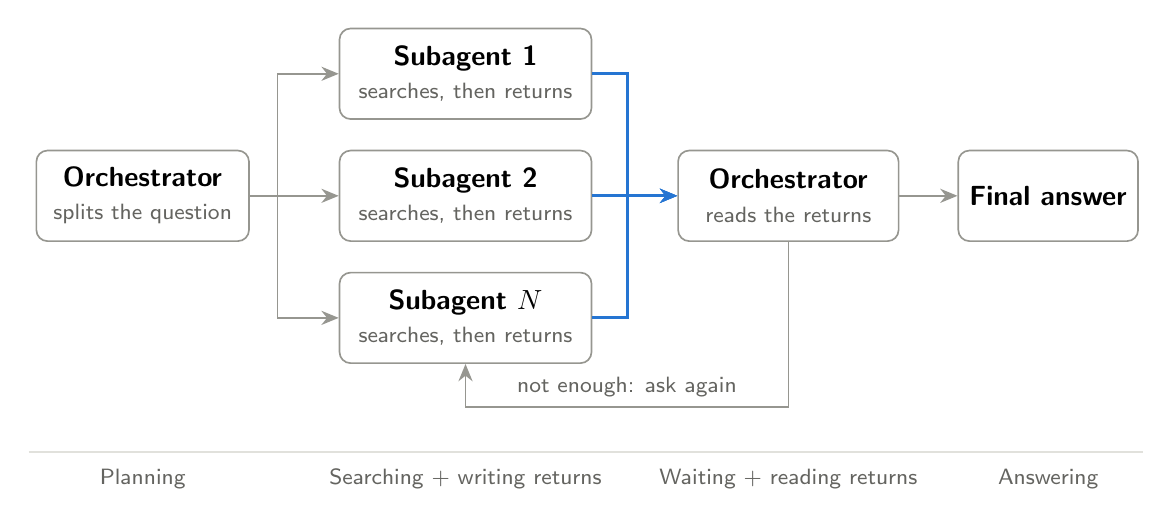
\begin{tikzpicture}[
  font=\sffamily,
  box/.style={draw=edge, line width=0.6pt, rounded corners=4pt, align=center,
              minimum height=1.15cm, inner sep=4pt},
  arr/.style={-{Stealth[length=2.2mm,width=1.8mm]}, draw=edge, line width=0.6pt},
  ret/.style={-{Stealth[length=2.2mm,width=1.8mm]}, draw=accent, line width=1.1pt},
  phase/.style={font=\sffamily\footnotesize, text=quiet},
]
  % Boxes
  \node[box, minimum width=2.7cm] (split) at (0,0)
    {\textbf{Orchestrator}\\{\footnotesize\color{quiet} splits the question}};
  \node[box, minimum width=3.2cm] (s1) at (4.1,1.55)
    {\textbf{Subagent 1}\\{\footnotesize\color{quiet} searches, then returns}};
  \node[box, minimum width=3.2cm] (s2) at (4.1,0)
    {\textbf{Subagent 2}\\{\footnotesize\color{quiet} searches, then returns}};
  \node[box, minimum width=3.2cm] (sn) at (4.1,-1.55)
    {\textbf{Subagent $N$}\\{\footnotesize\color{quiet} searches, then returns}};
  \node[box, minimum width=2.8cm] (read) at (8.2,0)
    {\textbf{Orchestrator}\\{\footnotesize\color{quiet} reads the returns}};
  \node[box, minimum width=2.2cm] (ans) at (11.5,0) {\textbf{Final answer}};

  % Dispatch from the orchestrator to the subagents
  \draw[arr] (split.east) -- ++(0.35,0) |- (s1.west);
  \draw[arr] (split.east) -- (s2.west);
  \draw[arr] (split.east) -- ++(0.35,0) |- (sn.west);

  % Returns (the variable under study), drawn in the accent color
  \draw[ret] (s1.east) -- ++(0.45,0) |- (read.west);
  \draw[ret] (sn.east) -- ++(0.45,0) |- (read.west);
  \draw[ret] (s2.east) -- (read.west);

  % Answer, or send subagents out again
  \draw[arr] (read.east) -- (ans.west);
  \draw[arr] (read.south) -- ++(0,-2.1) -| (sn.south)
    node[pos=0.25, above, font=\sffamily\footnotesize, text=quiet] {not enough: ask again};

  % Timed phases
  \draw[rule, line width=0.6pt] (-1.45,-3.25) -- (12.7,-3.25);
  \node[phase] at (0,-3.6)    {Planning};
  \node[phase] at (4.1,-3.6)  {Searching + writing returns};
  \node[phase] at (8.2,-3.6)  {Waiting + reading returns};
  \node[phase] at (11.5,-3.6) {Answering};
\end{tikzpicture}
}
  \caption{One run of the testbed. The orchestrator splits a question across $N$ subagents; each searches the corpus and returns its findings in one of six formats (blue arrows). Each labeled phase is timed separately. Written summaries cost time while subagents generate them; copied quotes and raw documents cost time while the orchestrator reads them.}
  \label{fig:system}
\end{figure}

Table~\ref{tab:formats} lists the six return formats we compare. Six formats at 1, 3 or 6 parallel subagents gives 18 configurations.

\begin{table}[!htbp]
  \centering\small
  \caption{The six return formats. The last column shows where each format spends its time.}
  \label{tab:formats}
  \begin{tabularx}{\linewidth}{@{}c P{2.9cm} L P{3.4cm}@{}}
    \toprule
    \textbf{\#} & \textbf{Format} & \textbf{What the subagent sends back} & \textbf{Who pays the time} \\
    \midrule
    1 & Short summary     & About 200 tokens of written summary & Subagent writing \\
    2 & Medium summary    & About 1,000 tokens (today's common default) & Subagent writing \\
    3 & Long summary      & About 3,000 tokens & Subagent writing \\
    4 & Structured claims & A short list of facts with evidence and document IDs, following PACT~\citep{huang2026pact} & Subagent writing (small) \\
    5 & Extracted quotes  & Document IDs plus exact passages, copied by the system, following Librarian~\citep{librarian2026} & Orchestrator reading \\
    6 & Raw documents     & The top documents found, untouched & Orchestrator reading \\
    \bottomrule
  \end{tabularx}
\end{table}

% =====================================================================
\section{Evaluation and Success Metric}
Every run logs its full trace, so each metric in Table~\ref{tab:metrics} can be recomputed later.

\begin{table}[!htbp]
  \centering\small
  \caption{Metrics captured for every run.}
  \label{tab:metrics}
  \begin{tabularx}{\linewidth}{@{}L P{5.6cm}@{}}
    \toprule
    \textbf{Metric} & \textbf{What it tells us} \\
    \midrule
    Answer accuracy (LLM judge, official BrowseComp-Plus grading~\citep{chen2025browsecompplus}) & Did the system get it right? \\
    Evidence recall: share of labeled evidence documents that reached the orchestrator & How much information each format loses \\
    Re-delegation rate & Whether short returns cause extra rounds \\
    End-to-end time per question & The latency users feel \\
    Time breakdown: subagent writing, orchestrator reading, waiting on the slowest subagent, extra rounds & Where the time goes under each format \\
    GPU-seconds per correct answer & Accuracy and cost in one number \\
    \bottomrule
  \end{tabularx}
\end{table}

\paragraph{Protocol.}
\begin{itemize}
  \item \textbf{Accuracy runs:} 200 questions $\times$ 18 configurations $\times$ 2 repeats, run at full throughput. Key configurations also run on all 830 questions.
  \item \textbf{Latency runs:} 100 questions $\times$ 18 configurations at a fixed, light load, so a busy server does not distort timing.
  \item \textbf{Comparisons:} the 1,000-token summary (today's default) is the reference point, plus a single-agent baseline. Configurations are compared on the same questions with paired tests.
\end{itemize}

\paragraph{Success metric.} The main result is a chart of accuracy against end-to-end time, one point per configuration.
\begin{itemize}
  \item \textbf{Target:} a format that stays within 2 points of the 1,000-token summary's accuracy while cutting end-to-end time by 20\% or more.
  \item \textbf{Minimum:} clean, repeatable measurements that confirm or reject H1 to H3 with confidence intervals. A tight ``no meaningful difference'' is still a useful result.
\end{itemize}

% =====================================================================
\section{Plan}
\subsection{Division of Labor}
Table~\ref{tab:labor} lists who leads each area. All four members share the pilot, the presentations and the writing.

\begin{table}[!htbp]
  \centering\small
  \caption{Division of labor.}
  \label{tab:labor}
  \begin{tabularx}{\linewidth}{@{}P{2.2cm}LL@{}}
    \toprule
    \textbf{Member} & \textbf{Leads} & \textbf{Also helps with} \\
    \midrule
    Person 1 & Agent harness and the six return formats & Prior work, writing \\
    Person 2 & Model serving and timing instrumentation & Latency runs \\
    Person 3 & Evaluation pipeline and accuracy runs & Grading, evidence recall \\
    Person 4 & Analysis, statistics and figures & Final report \\
    \bottomrule
  \end{tabularx}
\end{table}

\subsection{Milestones and Timeline}
Two checkpoints anchor the plan:
\begin{itemize}
  \item \textbf{By the mid-term report (Nov 5):} setup and single-agent baseline (Oct 9 to 18); testbed with all six return formats and per-phase timing (Oct 12 to 31); pilot across all 18 configurations to lock the design (Oct 26 to 31).
  \item \textbf{By the final report (Dec 9):} accuracy and latency runs (Nov 6 to 21); analysis (Nov 16 to 30); final talk (Dec 1 to 8); report, code and timed traces released (Dec 9).
\end{itemize}

% =====================================================================
\bibliographystyle{unsrtnat}
\bibliography{references}

\end{document}
